\documentclass[12pt,a4paper,ngerman,enabledeprecatedfontcommands]{scrreprt}

\usepackage[left=2.50cm, right=2.50cm, bottom=2.50cm, top=2.50cm]{geometry}
\usepackage[utf8]{inputenc}
\usepackage[german]{babel} 
\usepackage{natbib}
\usepackage{graphicx}
\usepackage[hyperfootnotes=false, hidelinks]{hyperref}
\usepackage[toc,section=section, numberedsection, nonumberlist]{glossaries}
%\usepackage{tabularx}
\usepackage{tabu}
\usepackage{listings}
\usepackage[nameinlink]{cleveref}
\usepackage{float}
\usepackage[compact]{titlesec}
\usepackage[table]{xcolor}
\usepackage{svg}
\usepackage{titling}
\usepackage{nameref}
\usepackage{wasysym}
\usepackage{pifont}
\usepackage{verbatim}
\usepackage{textcomp}
\usepackage{stmaryrd}
\usepackage{etoolbox}
\usepackage{xpatch}
\usepackage{siunitx}
\usepackage{stringstrings}
\usepackage{chngcntr}
\usepackage[all]{hypcap}
\usepackage{pdfpages}
\usepackage{tablefootnote}
\usepackage{lscape}
\usepackage{eurosym}
\usepackage{xcolor}
%\usepackage{comment}

% Erlaubt redefinieren dieser Befehle, behebt Konflikte
\makeatletter
    \let\diameter\relax
    \let\leftmoon\relax
    \let\rightmoon\relax
    \let\newmoon\relax
    \let\fullmoon\relax
\makeatother
\usepackage{mathabx}

% Hebt Kapiteltitel
\setlength{\droptitle}{-10em}

% Macht Fußnoten nach Zeilenumbruch linksbündig
\deffootnote[1em]{1em}{1em}{\textsuperscript{\thefootnotemark}}

% nummeriert im Inhaltsverzeichnis nur bis subsection
\setcounter{tocdepth}{2}
\setcounter{secnumdepth}{2}

%\hypersetup{
%    linkcolor=red,
%    urlcolor=black
%}

% streckt Tabellenzellen
\tabulinesep =3pt

% Verhindert, dass Fußnoten pro Kapitel von vorne nummeriert werden
\counterwithout*{footnote}{chapter}

\lstset
        {
            basicstyle=\small\ttfamily,
            breaklines=true,
            backgroundcolor = \color{gray!10},
            xleftmargin = 0.48cm,
            framexleftmargin = 1em
        }
        
\titleformat{\chapter}{\vspace{-2.5cm}\bf\huge}{\thechapter.}{20pt}{\bf\huge}

\renewcommand{\labelitemi}{$\RHD$}
\renewcommand{\labelitemii}{$\blacktriangleright$}

\addtokomafont{disposition}{\rmfamily}

\addtokomafont{descriptionlabel}{\rmfamily}

\setlength{\fboxsep}{0pt}%
\setlength{\fboxrule}{1pt}

\setlength{\parindent}{0pt}

\sisetup{   locale=DE,%
            round-mode=places,%
            round-precision=2,%
            per-mode=fraction%
}

\let\texteuro\euro

\DeclareSIUnit[per-mode=fraction]\schild{Schilder}
\DeclareSIUnit[per-mode=fraction]\PS{PS}

% Plus and Minus
\def\Plus{\texttt{+}}
\def\Minus{\texttt{-}}

% Table Highlights
\def\hl{\cellcolor[HTML]{DDDDDD}}

\let\subsubsubsection\paragraph

% Checkmark
\newcommand{\cmark}{\ding{51}}

\newcommand{\twodigit}[1]{\ifnum#1<10 0#1\else#1\fi}

% Links
\newcommand{\link}[1]{\href{#1}{#1}}
\newcommand{\footlink}[2]{\footnote{\href{#1}{\text{#1}}, #2}}
\newcommand{\footlinklabel}[3]{\footnote{\label{#3}\href{#1}{\text{#1}}, #2}}

\newcommand{\footlinktext}[2]
{
    \stepcounter{footnote}
    \footnotetext{\href{#1}{\text{#1}}, #2}
}

\newcommand{\footrealtext}[1]
{
    \stepcounter{footnote}
    \footnotetext{\text{#1}}
}

\newcommand{\linebar}
{
    \par\noindent\rule[\baselineskip]{\textwidth}{0.4pt}
}

%%%%%%%%%%%%%%%%%%%%%%%%%%%%%%%%%%%%%%%%%%%%%%%%%%%%%%%%%%%%%%%%%%%%%%%%%%%%%%%%%%%%%
% MuSCoW Naming                                                                     %
%%%%%%%%%%%%%%%%%%%%%%%%%%%%%%%%%%%%%%%%%%%%%%%%%%%%%%%%%%%%%%%%%%%%%%%%%%%%%%%%%%%%%

%\newcommand{\must}[1]{$\llbracket$#1$\rrbracket$}
%\newcommand{\should}[1]{$[$#1$]$}
%\newcommand{\could}[1]{$($#1$)$}
%\newcommand{\wont}[1]{$!$#1$!$}

\newcounter{musts}
\setcounter{musts}{0}
\newcounter{shoulds}
\setcounter{shoulds}{0}
\newcounter{coulds}
\setcounter{coulds}{0}
\newcounter{wonts}
\setcounter{wonts}{0}

\newcounter{chaprequirements}
\setcounter{chaprequirements}{0}

\newcommand*{\currentchapter}{Not set yet.}

\makeatletter
\xpretocmd{\@chapter}
{%
    \renewcommand*{\currentchapter}{#1}%
    \setcounter{chaprequirements}{0}%
}{}{}
\makeatother

\makeatletter
\xpretocmd{\section}
{%
    \setcounter{chaprequirements}{0}%
}{}{}
\makeatother

\newcommand*{\chaplet}{\substring[v]{\currentchapter}{1}{1}}
\newcommand*{\chapnum}{\substring[v]{\thesection}{1}{1}}
\newcommand*{\secnum}{\substring[v]{\thesection}{3}{3}}
\newcommand*{\reqcount}{\twodigit{\thechaprequirements}}

\newcommand*{\IDcode}{\chaplet\chapnum\secnum\reqcount}

\newcommand*{\musttext}{$\llbracket$\IDcode$\rrbracket$}
\newcommand*{\shouldtext}{$[$\IDcode$]$}
\newcommand*{\couldtext}{$($\IDcode$)$}
\newcommand*{\wonttext}{$!$\IDcode$!$}

\newcommand*{\must}
{%
    \refstepcounter{musts}%
    \stepcounter{chaprequirements}%
    \musttext%
    %\label{#1}%
}

\newcommand*{\should}
{%
    \refstepcounter{shoulds}%
    \stepcounter{chaprequirements}%
    \shouldtext%
    %\label{#1}%
}

\newcommand*{\could}
{%
    \refstepcounter{coulds}%
    \stepcounter{chaprequirements}%
    \couldtext%
    %\label{#1}%
}

\newcommand*{\wont}
{%
    \refstepcounter{wonts}%
    \stepcounter{chaprequirements}%
    \wonttext%
    %\label{#1}%
}

\newcommand*{\mustref}[1]
{%
    $\llbracket$#1$\rrbracket$%
}

\newcommand*{\shouldref}[1]
{%
    $[$#1$]$%
}

\newcommand*{\couldref}[1]
{%
    $($#1$)$%
}

\newcommand*{\wontref}[1]
{%
    $!$#1$!$%
}

\newcommand{\accref}[1]
{%
    $/$#1$/$%
}

%\crefname{musts}{}{}
%\creflabelformat{musts}{%
%   \addtocounter{chaprequirements}{-1}%
%    \musttext%
%    intern: #1
%    \addtocounter{chaprequirements}{1}%
%}
%
%\crefname{shoulds}{}{}
%\creflabelformat{shoulds}{%
%    \addtocounter{chaprequirements}{-1}%
%    \shouldtext%
%    intern: #1
%    \addtocounter{chaprequirements}{1}%
%}
%\crefname{coulds}{}{}
%\creflabelformat{coulds}{%
%    \addtocounter{chaprequirements}{-1}%
%    \couldtext%
%    intern: #1
%    \addtocounter{chaprequirements}{1}%
%}
%\crefname{wonts}{}{}
%\creflabelformat{wonts}{%
%    \addtocounter{chaprequirements}{-1}%
%    \wonttext%
%    intern: #1
%    \addtocounter{chaprequirements}{1}%
%}

\makenoidxglossaries
% https://alphabetizer.flap.tv/

\newglossaryentry{API}{name={API}, description={Application Programming Interface.\\ Programmierschnittstelle}}

\newglossaryentry{App}{name={App}, description={Application.\\Programm, welches auf einem Smartphone ausgeführt werden kann. Hier im Besonderen: Ein Teil des von uns entwickelten Produkts als Benutzerschnittstelle}}

\newglossaryentry{ALU}{name={ALU}, 
description={Arithmetic Logic Unit.\\ Das elektronische Rechenwerk eines Prozessors. Es ist speziell konzipiert um mathematische Operationen hocheffizient und schnell durchzuführen}}

\newglossaryentry{ARM}{name={ARM},
description={Acorn RISC Machine, bzw. Advanced RISC Machine.\\ Eine weit verbreitete Mikroprozessorarchitektur, welche sehr oft innerhalb von \gls{SoC}s in \gls{Smartphone}s zum Einsatz kommt}}

\newglossaryentry{CPU}{name={CPU}, 
description={Central Processing Unit.\\ Zentrales Rechen- und Steuerwerk einer Rechenmaschine, hier insb. eines Personalcomputers oder eines Smartphones}}

\newglossaryentry{Data Member}{name={Data Member}, description={~\\Klasseneigenschaft bzw. Membervariable. Eine Variable, die einer Instanz einer Klasse zugeordnet ist und von Instanz zu Instanz variieren kann}}

\newglossaryentry{Deep Learning}{name={Deep Learning}, description={~\\Klasse von Optimierungsmethoden Neuronaler Netzwerke, die zahlreiche Zwischenlagen zwischen Eingabeschicht und Ausgabeschicht haben und dadurch eine umfangreiche innere Struktur besitzen}}

\newglossaryentry{Drehachsen}{name={Drehachsen}, description={~\\Achsen, um die das Smartphone gedreht werden kann. Es gibt die Roll-, Gier- und Nickachse. \begin{figure}[H]
\centering
\includegraphics[width=0.5\linewidth]{Reviewdokument/Grafiken/drehachsen.png}
\end{figure}}}

\newglossaryentry{Detektion}{name={Detektion}, description={~\\Lokalisierung eines Merkmals (insb. eines Verkehrszeichens) in einem Bild}}

\newglossaryentry{Fahrzeug}{name={Fahrzeug}, description={~\\Handelsüblicher Personenkraftwagen (PKW), insbesondere kein Lastkraftwagen\\ (LKW)}}

\newglossaryentry{Filter}{name={Filter}, description={~\\Ein Verarbeitungsschritt. Jeder Filter hat eine Dateneingabe und eine -ausgabe. In jedem Verarbeitungsschritt werden die einkommenden Daten umgewandelt. Bei der Umwandlung können den Daten Teile entnommen, hinzugefügt oder auch vollständig ersetzt werden. Die Art der Umwandlung wird durch den Filter bestimmt}}

\newglossaryentry{Filterverwaltungs-Bibliothek}{name={Filterverwaltungs-Bibliothek}, description={~\\Programm-Bibliothek, welche Möglichkeiten bietet, Filter und Neuronale Filter zu laden und auf Bildserien anzuwenden}}

\newglossaryentry{FLOPs}{name={FLOPs}, 
description={Floating Point Operations.\\Operationen auf Fließkommazahlen, die von der \gls{ALU} ausgeführt werden. Sie gelten als eine der aufwendigsten, elementaren Operationen und bestimmen maßgeblich die Laufzeit eines Programms. Ausdrücklich zu unterscheiden von \glqq FLOPS\grqq}}

\newglossaryentry{FLOPS}{name={FLOPS}, 
description={Floating Point Operations per Second.\\Maß für die Leistungsfähigkeit von Computern. Ausdrücklich zu unterscheiden von \glqq FLOPs\grqq}}

\newglossaryentry{Geschwindigkeitsschild}{name={Geschwindigkeitsschild}, description={~\\Gibt die zulässige Höchstgeschwindigkeit des Fahrzeugs an, an dessen Rückseite es befestigt ist. Siehe §58 \gls{StVZO}}}

\newglossaryentry{GPU}{name={GPU}, 
description={Graphics Processing Unit; Grafikkarte.\\ Rechen- und Steuerwerk einer Rechenmaschine, hier insb. eines Personalcomputers oder eines Smartphones, welches auf die Bildverarbeitung spezialisiert ist}}

\newglossaryentry{Keras}{name={Keras}, description={~\\Deep-Learning-Framework in Python basierend auf TensorFlow}}

\newglossaryentry{Klassifikation}{name={Klassifikation}, description={~\\Einteilung eines Merkmals in eine Klasse von Urbildern}}

\newglossaryentry{Konfidenz}{name={Konfidenz}, description={~\\Sicherheit, dass das Objekt korrekt klassifiziert wurde}}

\newglossaryentry{Label}{name={Label}, description={~\\ Meta-Informationen zu einem Sample. In diesem Zusammhang die Position, Größe und Art von Verkehrsschildern in einer Bildaufnahme}}

\newglossaryentry{mAP}{name={mAP}, description={mean Average Precision.\\Maß für die Genauigkeit eines Objekt-Detektors und -Klassifikators. Basiert auf der Position und Größe des vermuteten Bildausschnitts sowie der Rangverteilung der vermuteten Klasse}}

\newglossaryentry{Multithreading}{name={Multithreading}, description={Nebenläufigkeit.\\ Gleichzeitiges Abarbeiten mehrerer Threads innerhalb eines Prozesses}}

\newglossaryentry{Neuronaler Filter}{name={Neuronale Filter}, description={~\\Ein Filter, dessen Umwandlungsvorgehen durch ein Neuronales Netz bestimmt wird}}

\newglossaryentry{Neuronales Netzwerk}{name={Neuronales Netzwerk}, description={~\\Hier im Besonderen: Künstliches Neuronales Netzwerk. Simplifiziertes Modell eines Nervensystems, bestehend aus künstlichen Neuronen, welche auf Computern trainiert werden, um komplexe Aufgaben im Bereich der künstlichen Intelligenz zu bewältigen}}

\newglossaryentry{Nutzer}{name={Nutzer}, description={~\\Der aktuelle Fahrzeugführer, während sich das Fahrzeug nicht in Fahrt befindet bzw. der Beifahrer, während sich das Fahrzeug in Fahrt befindet. Es wird das generische Maskulinum verwendet}}

\newglossaryentry{OpenCV2}{name={OpenCV2}, description={Open Source Computer Vision Library. \\Quelloffene Computergrafikbibliothek. Hier verwendet um Datensätze sowie das erfasste Kamerabild auf die Eingabespezifikationen der Neuronalen Netzwerke anzupassen}}

\newglossaryentry{Produkt}{name={Produkt}, description={~\\Die Kombination aus App und API, welche im Rahmen dieses Softwareprojektes entwickelt werden}}

\newglossaryentry{Pipe}{name={Pipe}, description={~\\Eine Pipe stellt eine Verbindung zwischen den einzelnen Verarbeitungsschritten dar}}

\newglossaryentry{Pipes and Filters}{name={Pipes and Filters}, description={auch Datenfluss-System.\\ Ein Architekturmuster welches die Struktur für Systeme, die Datenströme verarbeiten, darstellt}}

\newglossaryentry{Protobuf}{name={Protocol Buffers, Protobuf}, description={~\\Bezeichnet ein von Google entwickeltes, programmiersprachen- und plattformunabhängiges Format sowie die dazugehörige Implementierung für die Serialisierung und Deserialisierung strukturierter Daten.}}

\newglossaryentry{Sample}{name={Sample}, description={~\\In diesem Zusammenhang eine Bildaufnahme von Verkehrszeichen, welche Neuronalen Netzwerken präsentiert werden können, um sie zur Detektion und Klassifkation zu trainieren}}

\newglossaryentry{Smartphone}{name={Smartphone}, description={~\\Mobiles Endgerät, welches über eine integrierte Kamera verfügt und den im Pflichtenheft spezifizierten Bedingungen genügt}}

\newglossaryentry{SoC}{name={SoC}, description={System-on-a-Chip.\\ Kombination von CPU, Bus, Taktgeber, Co-CPUs, GPU, Soundchip, Interfaces, etc. oder Teilen davon auf einem Chip. Häufig verwendet in mobilen Endgeräten und eingebetteten Systemen um durch hohe Integrationsdichten Fläche auf der Platine einzusparen}}

\newglossaryentry{StVO}{name={StVO}, description={Straßenverkehrsordnung\footlink{https://www.gesetze-im-internet.de/stvo\_2013/StVO.pdf}{29.04.2018}}}

\newglossaryentry{StVZO}{name={StVZO}, description={Straßenverkehrszulassungsordnung\footlink{https://www.gesetze-im-internet.de/stvzo\_2012/StVZO.pdf}{29.04.2018}}}

\newglossaryentry{System}{name={System}, description={~\\Gesamtheit aus Halterung, Smartphone und App}}

\newglossaryentry{Tracking}{name={Tracking}, description={~\\Objekte anhand primitiver Merkmale in einer Bildserie oder einem Video lokalisieren und verfolgen}}

\newglossaryentry{TensorFlow Lite}{name={TensorFlow Lite}, description={~\\Für mobile Endgeräte optimiertes Deep-Learning-Framework des Google Brain Teams\footlink{https://www.tensorflow.org/mobile/tflite/}{29.04.2018}}}

\newglossaryentry{TensorFlow Mobile}{name={TensorFlow Mobile}, description={~\\Deep-Learning-Framework des Google Brain Teams, welches zwar für Android noch keine GPU Unterstützung bietet, dafür aber derzeit noch bzgl. der Kompatibilität besser von bereits etablierten Netzwerken unterstützt wird}}

\newglossaryentry{Tensorflow Node}{name={Tensorflow Node},description={~\\Ein Knoten (Node) im Sinne von TensorFlow bezeichnet eine bestimmte Operation innerhalb des Netzwerk Models: Es ist die grundlegende Einheit für Berechnungen innerhalb von TensorFlow. Die Ergebnisse dieser Knoten lassen sich anhand deren Bezeichnungen (zum Beispiel \glqq{}final\_output\qrqq{})  einzeln abfragen}}

\newglossaryentry{UI}{name={UI},description={User Interface.\\ Benutzeroberfläche}}

\newglossaryentry{VZ}{name={VZ}, description={Verkehrszeichen}}

\newglossaryentry{Verkehrszeichen-API}{name={Verkehrszeichen-API}, description={~\\Besondere Programmierschnittstelle, die für Verkehrszeichenerkennung optimiert ist und erweiterte Logik zur Verfügung stellt, wie etwa die Abschätzung, wann ein Verkehrsschild passiert wurde und damit gültig ist und angezeigt werden muss}}

\newglossaryentry{Verkehrszeichenkombination}{name={Verkehrszeichenkombination}, description={~\\Gruppe von untereinander angebrachten Verkehrszeichen, welche einen gemeinsamen Sinnzusammenhang darstellen}}

\newglossaryentry{VwV-StVO}{name={VwV-StVO}, description={Allgemeine Verwaltungsvorschrift
zur Straßenverkehrs-Ordnung\footlink{http://www.verwaltungsvorschriften-im-internet.de/bsvwvbund\_26012001\_S3236420014.htm}{29.04.2018}}}



\author{
    [Projektgruppe 2]\\~\\
    \textit{Namen entfernt}\\~\\
    \textcolor{red}{Verwendung nur zu Lehrzwecken an der TU Ilmenau. Die Verwendung}\\\textcolor{red}{für private oder kommerzielle Zwecke ohne Einwilligung der Autoren ist}\\ \textcolor{red}{ausdrücklich untersagt.}\\~\\
    Kontakt: \href{mailto:signapse.app@gmail.com}{signapse.app@gmail.com}
    %Bock, Robert Niklas\\ \texttt{robert-niklas.bock@tu-ilmenau.de}\\~\\
    %Dirbas, Mohammad\\ \texttt{mohammad.dirbas@tu-ilmenau.de} \\~\\
    %Fischedick, Söhnke Benedikt\\ \texttt{soehnke-benedikt.fischedick@tu-ilmenau.de} \\~\\
    %Hampel, Jakob Frank\\ \texttt{jakob.hampel@tu-ilmenau.de} \\~\\
    %Köhler, Florian\\ \texttt{florian.koehler@tu-ilmenau.de} \\~\\
    %Langer, Patrick\\ \texttt{patrick.langer@tu-ilmenau.de} \\~\\
    %Nowati, Yusuf\\ \texttt{yusuf.nowati@tu-ilmenau.de} \\~\\
    %Treichel, Tim\\ \texttt{tim.treichel@tu-ilmenau.de} \\ ~\\ ~\\ ~\\ ~\\
}


\title{Pflichtenheft\\ Verkehrszeichenerkennung}

\date{~\\01.05.2018}

\begin{document}
\maketitle%
%\clearpage

\addtocounter{page}{-1}
\topskip0pt
\vspace*{\fill}

\begin{center}
%Dieses Dokument ist für die Verwendung mit %\href{https://get.adobe.com/de/reader/}{Adobe$^{\tiny{\text{\textregistered}}}$ %Reader$^{\tiny{\text{\textregistered}}}$} optimiert.\\
%\href{https://get.adobe.com/de/reader/}{https://get.adobe.com/de/reader/} \\
{\bfseries Temporärer Disclaimer!}\\
~\\
Dieses Dokument wurde zuletzt von Söhnke und Robert am 01.05.2018 um 23:44 Uhr auf Rechtschreib-, Grammatik-, Struktur-, Logik- und Crossreferencing-Fehler untersucht. Wer nach diesem Datum Änderungen durchführt ist für die Integrität selbst verantwortlich und wird von uns höchstpersönlich \underline{gelyncht}, wenn er es versäumt diese zu bewahren!\\
~\\
{\bfseries Vor Abgabe Entfernen!}\\
\end{center}
\vspace*{\fill}%
\tableofcontents%
%%%%%%%%%%%%%%%%%%%%%%%%%%%%
%%%%%%%%%%%%%%%%%%%%%%%%%%%%
% MANDATORY; DO NOT REMOVE %
%%%%%%%%%%%%%%%%%%%%%%%%%%%%
\pagestyle{plain}%%%%%%%%%%%
%%%%%%%%%%%%%%%%%%%%%%%%%%%%

\chapter{Zielbestimmungen}
\label{chap:zielbestimmmungen}

\section{Ausgangssituation}
Die meisten Autofahrer kennen das Gefühl der Unsicherheit über die aktuell erlaubte Höchstgeschwindigkeit. Daher verfügen viele moderne Fahrzeuge über eine automatische Verkehrszeichenerkennung, mit deren Hilfe der Fahrzeugführer zu jedem Zeitpunkt über die aktuell geltenden Verkehrsregelungen informiert ist. Der Fahrzeugführer kann beispielsweise stets die zulässige Geschwindigkeit nachvollziehen und gegebenenfalls auf ein Überschreiten dieser hingewiesen werden. Die Verkehrszeichenerkennung ist dabei meist als Fahrerassistenzsystem fest im \gls{Fahrzeug} verankert und nutzt zur Erkennung der Verkehrszeichen eine in Höhe des Innenspiegels angebrachte Kamera. Folglich ist ein solches Assistenzsystem ausschließlich modernen Fahrzeugen mit entsprechender Ausstattung vorbehalten.
Bisher existierte keine, mit diesem Projekt vergleichbare, praktikable Möglichkeit, ein solches Assistenzsystem auch in älteren und preisgünstigeren Fahrzeugen nachzurüsten. Zwar sind diverse Apps zur Verkehrszeichenerkennung für Android und iOS bereits verfügbar, allerdings ist keine davon in der Lage, mit der in diesem Projekt geplanten Verlässlichkeit und Performanz geschwindigkeitsregulierende Verkehrszeichen und \glslink{Verkehrszeichenkombination}{Verkehrszeichenkombinationen} zu erkennen.\\

\section{Ziel}
Ziel dieses Softwareprojektes ist es, ein \gls{System} (bestehend aus einem \gls{Smartphone}, einer KFZ-Smartphonehalterung und einer \gls{App}) zur Verkehrszeichenerkennung zu entwickeln,
welches in jedem \gls{Fahrzeug} nachgerüstet werden kann. Inhalt der dafür zu entwickelnden \gls{App} ist eine Benutzerschnittstelle, welche erkannte Verkehrszeichen während der Fahrt anzeigt, sowie eine Logik-Schnittstelle, welche in Echtzeit aus Kameraaufnahmen Verkehrsschilder identifiziert, aber derart modular aufgebaut ist, um auch andere Detektionsprobleme zu lösen.\\

\section{Musskriterien}
\label{sec:musskriterien}
Im Folgenden werden die Produkteigenschaften und -funktionen genannt, welche für das Projekt unabdingbar sind. Sollte eines dieser Kriterien nicht erfüllt werden können, kann das Endergebnis in seiner Nutzbarkeit sehr stark eingeschränkt sein.

\begin{itemize}

\item Die Verkehrszeichenerkennung soll bei klarer Sicht und Tageslicht bis zu einer maximalen Geschwindigkeit funktionieren.

\item Das \gls{System} soll unter genauer Spezifikation von Halterung und Spannungsversorgung für das \gls{Smartphone} in jedem \gls{Fahrzeug} nachgerüstet werden können.

\item Der \gls{Nutzer} soll zur richtigen Ausrichtung des \glslink{Smartphone}{Smartphones} bei Stillstand des Fahrzeugs mit einer Kalibrierungsphase unterstützt werden. Er soll dazu Anweisungen auf dem Bildschirm erhalten.

\item Die Erkennung von Verkehrszeichen, Zusatz- und Sonderschildern durch die \gls{App} ist auf solche beschränkt, welche einen Einfluss auf die minimal oder maximal zulässige Geschwindigkeit sowie ihren Geltungsbereich haben.

\item Die \gls{App} soll in der Lage sein, \glslink{Geschwindigkeitsschild}{Geschwindigkeitsschilder} (gemäß §58 \gls{StVZO}) auf LKWs herauszufiltern, um ein fehlerhaftes Anzeigen zu vermeiden.

\item Die Erkennung der Verkehrszeichen soll in Echtzeit, das heißt videotaktschritthaltend erfolgen. Nach dem Passieren eines Verkehrszeichens darf höchstens eine kaum bemerkbare Verzögerung bis zum Erscheinen auf dem Display entstehen.

\item Die Kernfunktionalität zur \gls{Detektion} und \gls{Klassifikation} von Verkehrszeichen im Kamerabild soll auf andere \glslink{Detektion}{Detektionsprobleme} übertragbar gestaltet sein. Dafür wird dieser Aspekt in eine eigene wiederverwendbare Bibliothek ausgelagert, im Folgenden \glqq\gls{Filterverwaltungs-Bibliothek}\grqq{} genannt.
\end{itemize}

\section{Sollkriterien}
Im Folgenden werden die Produkteigenschaften und -funktionen genannt, welche für das Projekt als Soll-Anforderung gelistet sind. Sollte eines dieser Kriterien nicht erfüllt werden, entspricht das \gls{Produkt} nicht mehr allen Anforderungen des Auftraggebers, ist aber dennoch nutzbar.

\begin{itemize}
\item Die aktuelle Geschwindigkeit soll nach Wunsch mittels GPS erfasst werden. Bei Überschreitung der zulässigen Geschwindigkeit - ermittelt aus dem aktuell erkannten Verkehrszeichen - wird eine entsprechende Warnung auf dem Display dargestellt.

\item Die Benutzeroberfläche soll sowohl in deutscher als auch englischer Sprache zur Verfügung stehen.

\item Die Erkennung soll mittels \glslink{Neuronales Netzwerk}{Neuronaler Netzwerke} realisiert werden.
\end{itemize}

\section{Wunschkriterien}
Im Folgenden werden die Produkteigenschaften und -funktionen genannt, welche für das Projekt als Kann-Anforderungen gelten. Die Erfüllung dieser Kriterien ist vom Auftraggeber nicht verpflichtend gefordert, allerdings gewünscht, da sie das \gls{Produkt} in seiner Nutzbarkeit deutlich aufwerten.

\begin{itemize}
\item Die \gls{App} soll auf \glslink{Smartphone}{Smartphones} mit mindestens iOS Version 10 (Whitetail) ausgeführt werden können.

\item Die \gls{App} soll ohne aktive Internetverbindung nutzbar sein.

\item Zusätzlich zur visuellen Warnung bei überhöhter Geschwindigkeit soll eine Sprachausgabe erfolgen.

\item Die \gls{App} soll Wechselverkehrszeichen zur Geschwindigkeitsregulierung erkennen können.

\item Zur Verbesserung der Erkennungsleistung und zur Korrektur von Fehlern sollen Informationen aus Kartendaten extrahiert und verwendet werden können.

\item Bei Verwendung einer anderen \gls{App}, beispielsweise zur Navigation, soll unter Android die Möglichkeit bestehen, die aktuell erkannten Verkehrszeichen über dieser einzublenden. Dazu muss die Verkehrszeichenerkennung im Hintergrund weiterlaufen können.

\end{itemize}

\section{Abgrenzungskriterien}
Im Folgenden werden die Grenzen des \glslink{Produkt}{Produktes} aufgelistet. Sie stellen Funktionen dar, die in diesem Projekt ausdrücklich nicht bearbeitet und ignoriert werden, um den Zeitaufwand zu begrenzen.
\begin{itemize}
    \item Die Funktionalität wird zu Zeiten mit Niederschlägen und Fahrten bei Nacht nicht garantiert.
    \item Die Funktionalität wird bei starker frontaler Sonneneinstrahlung, welche die Kamera blenden könnte nicht garantiert.
    \item Verkehrszeichen, welche auf die aktuelle Mindest- oder Höchstgeschwindigkeit keinen Einfluss haben, werden von der Erkennung nicht unterstützt.
\end{itemize}

\chapter{Produkteinsatz}
\label{chap:produkteinsatz}

\section{Zielgruppen}
\begin{itemize}
%\hline
\item Das \gls{System} soll von Fahrzeugführern mit Android-\gls{Smartphone} bzw. deren Beifahrern verwendet werden können.

%\hline
\item Die \gls{Filterverwaltungs-Bibliothek} soll von Anwendungs-Programmierern mit Erfahrung in Java und C++ verwendet werden können.
%\hline
\end{itemize}

\section{Betriebsbedingungen}
\label{sec:betriebsbedingungen}

\begin{itemize}

%\item Die App ist für den Dauerbetrieb, also unterbrechungsfreie 24 Stunden pro Tag, ausgelegt.

\item Die Verkehrszeichenerkennung der \gls{App} ist für Geschwindigkeiten bis zu 150km/h ausgelegt.

\item Das \gls{Smartphone}, auf welchem die \gls{App} ausgeführt wird, muss an der Windschutzscheibe bzw. in der Nähe der Windschutzscheibe auf dem Armaturenbrett des Fahrzeugs montiert werden. Die Kamera muss ein freies Sichtfeld auf den Verkehr besitzen und in einem von der \gls{App} festgelegten Winkel auf die Fahrbahn zeigen. Damit dies erreicht werden kann, soll es eine Anleitung zur Ausrichtung in der \gls{App} geben.

\item Die zu erkennenden Verkehrszeichen müssen gemäß \gls{VwV-StVO} §§ 39-43 aufgestellt sein und sich im Originalzustand befinden.

\item Die Verkehrszeichenerkennung wird nur bei Tag und bei klarer Sicht (kein Nebel, kein Niederschlag, kein starkes Gegenlicht) garantiert. (Unter diesen Umständen und einem dunklen Armaturenbrett stellen Spiegelungen an der Frontscheibe kein Problem dar.)

\item Um eine dauerhafte Nutzung zu gewährleisten, muss das \gls{Smartphone} mit einem ausreichend starken Ladegerät verbunden sein. Der verwendete USB-Port sollte erfahrungsgemäß mindestens 2A bei 5V liefern. Die meisten in Autos integrierten USB-Anschlüsse liefern allerdings nicht diese Leistung. Deshalb sollte stattdessen ein KFZ-Ladeadapter mit entsprechend beschriebenen Leistungsfähigkeiten verwendet werden. Das Ladekabel muss zudem in der Lage sein, die beschriebene Leistung zu übertragen. Es ist deshalb empfehlenswert, das Original-Ladekabel oder ein entsprechend der Leistung ausreichend spezifiziertes Kabel zu verwenden. Ein guter Indikator für nicht ausreichende Ladeleistung ist ein abnehmender Ladestand trotz angeschlossenem Ladegerät.

\item Der Stromverbrauch des \glslink{Smartphone}{Smartphones} kann verringert werden, indem beispielsweise das Display maximal bei halber Helligkeit gehalten, im Hintergrund laufende Apps wie z.B. Musikwiedergabe beendet oder Funkverbindungen wie WLAN, Bluetooth oder NFC deaktiviert werden. Bei Bedarf kann die Helligkeit weiter reduziert oder ein anderes Ladegerät und/oder Kabel mit besseren Ladeeigenschaften genutzt werden.

\end{itemize}

\chapter{Produktumgebung}
\section{Software}
Als Betriebssystem muss auf dem \gls{Smartphone} Android, ab Version 7.0 (Nougat, \gls{API} Version 24), installiert sein.\\
Eine Portierung auf iOS, ab Version 10.0 (Whitetail), ist optional geplant.\\
\\
Des Weiteren wird das \glslink{Deep Learning}{Deep-Learning}-Framework \glqq \gls{TensorFlow Lite}\grqq{} benötigt, welches direkt in die \gls{App} eingebunden ist, um diese Abhängigkeit bei der Installation zu erfüllen.\\

\section{Hardware}
\label{chap:hardware}
Als Hardwareumgebung wird ein \gls{Smartphone} vorausgesetzt, welches 2016 oder später veröffentlicht wurde.\\
Das Gerät muss über einen GPS-Empfänger sowie eine integrierte Kamera mit Bildstabilisierung verfügen.
Außerdem soll es einen Qualcomm Snapdragon \gls{SoC} der 600er oder 800er Series\footlink{https://www.qualcomm.com/snapdragon/processors/comparison}{27.04.2018} oder einen anderen mit vergleichbarer Leistung (z.B. vergleichbare \gls{SoC}s der Samsung Exynos Series\footlink{http://www.samsung.com/semiconductor/minisite/exynos/products/all-processors/}{27.04.2018}) besitzen. Weiterhin sollen dem Gerät mindestens 3 Gibibyte Arbeitsspeicher (RAM) zur Verfügung stehen und 512 Mebibyte Speicher frei sein.\\

\chapter{Produktfunktionen}
\label{chap:produktfunk}
Im Folgenden werden die generell geforderten, gewünschten und ausgeschlossenen Anforderungen an das \gls{System} beschrieben. Dabei wird die hier beschriebene Notation zur Markierung des Anforderungstyps verwendet:

\begin{longtabu}{l X[l]}
\mustref{~} & Muss-Anforderung\\
&\\
\shouldref{~} & Soll-Anforderung\\
&\\
\couldref{~} & Kann-Anforderung\\
&\\
\wontref{~} & Abgrenzung\\
&\\
\end{longtabu}

\section{Zu erkennende Verkehrszeichen}
\begin{longtabu}{l X[j]}

\must & Das \gls{System} soll unter den in \cref{sec:betriebsbedingungen} beschriebenen Betriebsbedingungen die im \cref{sec:liste_zu_erkennende_verkehrszeichen} spezifizierten Verkehrszeichen erkennen können.\\
&\\
\must & Das System soll in der Lage sein, ein \gls{Geschwindigkeitsschild}, welches gemäß \gls{StVZO} § 58 an einem voranfahrendem \gls{Fahrzeug} angebracht ist, als solches zu erkennen und herauszufiltern.\\
&\\
\could & Das System kann Wechselverkehrszeichen zur Geschwindigkeitsregulierung erkennen.\\
&\\
\wont & Verkehrszeichen, welche keinen Einfluss auf die erlaubte Geschwindigkeit haben und damit nicht in \cref{sec:liste_zu_erkennende_verkehrszeichen} gelistet sind, werden nicht erkannt oder angezeigt.\\
&\\

\end{longtabu}

\section{Bereitgestellte Funktionen der Filterverwaltungs-Bibliothek}
\begin{longtabu}{l X[j]}

\must & Die \gls{Filterverwaltungs-Bibliothek} erlaubt das Implementieren beliebiger \gls{Filter}, welche Modifikationen auf einer Eingabe ausführen und diese danach für weitere Modifikatonen freigeben.\\
&\\
\must & Die \gls{Filterverwaltungs-Bibliothek} stellt die grundlegenden Funktionen für die Verwendung von \glslink{Filter}{Filtern} und \glslink{Neuronaler Filter}{Neuronalen Filtern}, also \gls{Filter} welche auf \glslink{Neuronales Netzwerk}{Neuronalen Netzwerken} basieren, bereit.\\
&\\
\must & Die \gls{Filter} können einer \gls{Pipe}, also einer Datenverarbeitungsstrecke, hinzugefügt werden. Es ist dabei möglich, mehrere \glslink{Pipe}{Pipes} anzulegen. Ein eingegebenes Bild wird durch selbige verarbeitet.\\
&\\
\should & Es kann konfiguriert werden, ob bestimmte \gls{Filter}, sofern möglich, echt parallel durch \gls{Multithreading} abgearbeitet werden sollen.\\
&\\
\end{longtabu}

\section{Funktionen der App}
Anforderungen an die Benutzeroberfläche werden später in \cref{chap:ui} beschrieben.\\

\begin{longtabu}{l X[j]}

\must & Die \gls{App} soll Kamerabilder aufnehmen und diese mittels der \gls{Filterverwaltungs-Bibliothek} auf Verkehrszeichen, beziehungsweise auf \glslink{Verkehrszeichenkombination}{Verkehrszeichenkombinationen} untersuchen.\\
&\\
\must & Alle erkannten \glslink{Verkehrszeichenkombination}{Verkehrszeichenkombinationen} sollen zeitlich geordnet und in der maximalen Anzahl begrenzt in einer Historie bis zum Beenden der \gls{App} gespeichert werden.\\
&\\
\should & Es soll möglich sein, die maximale Anzahl an \glslink{Verkehrszeichenkombination}{Verkehrszeichenkombinationen}, welche in der Historie aus \mustref{P4302} gehalten werden, festzulegen.\\
&\\
\should & Die \gls{App} soll in der Lage sein, mittels GPS-Ortung die aktuelle Fahrgeschwindigkeit zu ermitteln.\\
&\\
\should & Die Funktion zur Geschwindigkeitsermittlung nach \shouldref{P4304} soll ein- und ausschaltbar sein.\\
&\\
\must & Die \gls{App} soll über eine interaktive Anleitung zur Justierung des \glslink{Smartphone}{Smartphones} in der Halterung verfügen.\\
&\\
\must & Die \gls{App} soll zu Beginn der Verwendung dem \gls{Nutzer} eindeutig vermitteln, dass sie kein Ersatz für die eigene Aufmerksamkeit am Steuer ist und dass deren Anwendung nur innerhalb der geltenden \gls{StVO} erfolgen darf.\\
&\\
\could & Die \gls{App} soll in der Lage sein, zur Verbesserung der Erkennungsleistung und zur Korrektur von Fehlern Informationen aus Kartenmaterial zu extrahieren und anzuwenden.\\
&\\
\end{longtabu}


%Nicht-Funktionale Anforderungen
\chapter{Produktleistungen}
Im Folgenden wird die Notation aus \cref{chap:produktfunk} weiter verwendet.\\

\begin{longtabu}{l X[l]}

\must & Der Prozess der Verkehrszeichenerkennung soll unter Einhaltung der in \cref{chap:hardware} beschriebenen Hardwareanforderungen vom Vorbeifahren am Verkehrszeichen bis zur Anzeige auf dem Bildschirm des \glslink{Smartphone}{Smartphones} maximal eine Sekunde in Anspruch nehmen.\\
&\\
\must & Die erfolgreiche Verkehrszeichenerkennung kann nur bei den unter \cref{sec:betriebsbedingungen} und \cref{chap:hardware} beschriebenen Bedingungen und Hardwareanforderungen verlässlich garantiert werden.\\
&\\
\could & Bei Verwendung einer anderen \gls{App}, beispielsweise zur Navigation, soll unter Android die Möglichkeit bestehen, die aktuell erkannten Verkehrszeichen über dieser einzublenden. Dazu muss die Verkehrszeichenerkennung im Hintergrund weiterlaufen können.\\
&\\
\should & Die \gls{App} soll ohne aktive Internetverbindung funktionieren. Im Fall der Umsetzung von \couldref{P4308} ist diese Anforderung außer Kraft gesetzt.\\
&\\
\must & Die \gls{Filterverwaltungs-Bibliothek} soll modular gestaltet sein, so dass sie auf beliebige \glslink{Detektion}{Detektionsprobleme} übertragen werden kann.\\
&\\
\should & Für Kernfunktionalität und Oberfläche soll eine Trennung in Hinblick auf eine Portierung für das Betriebssystem iOS erfolgen.\\
&\\
\end{longtabu}


\chapter{Benutzeroberfläche}
\label{chap:ui}
Im Folgenden wird die Notation aus \cref{chap:produktfunk} weiter verwendet.\\

\begin{longtabu}{l X[l]}
\must & Die zuletzt erkannte \gls{Verkehrszeichenkombination} soll präsent in der \gls{App} dargestellt werden (siehe \cref{fig:ui_det} links).\\
&\\
\must & Auf dem Display soll neben \mustref{B6001} eine Auswahl der Einträge aus der Historie angezeigt werden (siehe \cref{fig:ui_det} rechts), welche durch eine Wisch-Geste geändert werden kann.\\
&\\
\must & Bei der Darstellung von \glslink{Verkehrszeichenkombination}{Verkehrszeichenkombinationen} auf dem Display soll jeweils die vergangene Zeit seit dem Erkennen mit angezeigt werden (siehe \cref{fig:ui_det} unten).\\
&\\
\should & Wird die Geschwindigkeit nach \shouldref{P4305} ermittelt, soll die \gls{App} eine visuelle Warnung bei erkannter Geschwindigkeitsüberschreitung (zum Beispiel bei Verstoß gegen \gls{VZ} 274) darstellen.\\
&\\
\could & Wird die Geschwindigkeit nach \shouldref{P4305} ermittelt, soll die \gls{App} eine visuelle Warnung bei erkannter Geschwindigkeitsunterschreitung (bei Verstoß gegen \gls{VZ} 275) darstellen.\\
&\\
\could & Zusätzlich zu der in \shouldref{B6004} und \couldref{B6005} beschriebenen visuellen Warnung soll ebenfalls eine ein- und ausschaltbare Sprachausgabe erfolgen.\\
&\\
\should & Zur optimalen Ausrichtung der Kamera ist die Verwendung der \gls{App} nur im Querformat, welcher als Landscape-Mode bezeichnet wird, vorgesehen. Die Benutzung im Hochformat (Portrait-Mode) ist nicht vorgesehen und wird dementsprechend nicht implementiert werden.\\
&\\
\should & Die Sprache der \gls{App} wird automatisch der Systemsprache des Gerätes angepasst. Die \gls{App} ist mit deutscher und englischer Oberfläche verfügbar, wobei im Falle einer von der \gls{App} nicht unterstützten Systemsprache standardmäßig Englisch übernommen wird.\\
&\\
\should & Im Falle einer eingeschalteten Geschwindigkeitsermittlung nach \shouldref{P4305} soll die Geschwindigkeit auf dem Display dargestellt werden (siehe \cref{fig:ui_det} unten links).\\
&\\
\end{longtabu}

\begin{figure}[H]
\centering
\includesvg[width=1\linewidth]{Grafiken/app_det_ls.svg}
\caption{Benutzeroberfläche Konzept}
\label{fig:ui_det}
\end{figure}

\chapter{Qualitätsbestimmungen}

Im Folgenden sei beschrieben, inwiefern nichtfunktionale Kriterien im Endprodukt von Relevanz sind. \\

\begin{longtabu}{|X[l]|c|c|c|}
\hline
\bf Qualitätsmerkmal & \bf essentiell & \bf bedeutend & \bf vernachlässigbar \\ 
\hline
&&&\\
Effizienz               &       &\cmark       &\        \\
&&&\\
\hline
&&&\\
Fehlertoleranz          &       &\cmark &              \\
&&&\\
\hline
&&&\\
Korrektheit             &\cmark &        &              \\
&&&\\
\hline
&&&\\
Nutzerfreundlichkeit    &       &\cmark       &        \\
&&&\\
\hline
&&&\\
Portierbarkeit          &\cmark       &       &        \\
&&&\\
\hline
&&&\\
(Informations-)\newline Sicherheit            && &\cmark \\
&&&\\
\hline
\end{longtabu}


%%%%%%%%%%%%%%%%%%%%%%%%%%%%%%%%%%%%%%%%%%%%%%%%%%%%%%%%%%%%%%%%%%%%%%%%%%%%%%%%%%%
% Kapitel 8
% ist ausgelagert
% später \pdfinclude
%%%%%%%%%%%%%%%%%%%%%%%%%%%%%%%%%%%%%%%%%%%%%%%%%%%%%%%%%%%%%%%%%%%%%%%%%%%%

\includepdf[landscape=true,pages=-,addtotoc={
     1,chapter,0,Abnahmekriterien und Testfälle,p1,   
     1,section,1,Abnahme für Produktfunktionen und Produktleistungen,p2,
     4,section,1,Beschreibung der Teststrecke,p3}]{Pflichtenheft/SubPDFs/Abnahmekriterien_und_Testfaelle.pdf}

\begin{comment}
\chapter{Realisierungsmodell}

\section{Produktstruktur}
Die \gls{App} dient im \gls{Produkt} vorwiegend als Benutzerschnittstelle, welche mit einer aufgeräumten und übersichtlichen Oberfläche dem \gls{Nutzer} Informationen über bisher erkannte Verkehrszeichen anzeigt. Außerdem bietet sie einen einfachen Zugang zur Kamera \gls{API} des \glslink{Smartphone}{Smartphones}.\\
Die Programm-Bibliothek basiert auf einer \glslink{Pipes and Filters}{\glqq Pipes \& Filters\grqq{}}-Architektur. Das bedeutet: Eingaben werden auf einem zentralen Kommunikationskanal transportiert und nacheinander durch einzelne \gls{Filter} verarbeitet. Hierbei stellt ein \gls{Filter} einen Algorithmus dar, welcher Modifikationen an der gegebenen Eingabe vornimmt und anschließend seine Ausgabe wieder auf die \gls{Pipe} legt, damit der nächste \gls{Filter} sie bearbeiten kann. Daher wird die Bibliothek ab sofort als \glqq{}\gls{Filterverwaltungs-Bibliothek}\grqq{} bezeichnet.\\
Der Algorithmus, den ein \gls{Filter} verwendet, kann auch von einem \glslink{Neuronales Netzwerk}{Neuronalen Netzwerk} realisiert werden. Daher werden im Folgenden solche speziellen \gls{Filter} als \glqq Neuronale Filter\grqq{} bezeichnet.\\ 
\\
Um mit dem \gls{Produkt} die gewünschte Erkennung zu realisieren, werden mittels der \gls{App} kontinuierlich Kamerabilder geschossen, welche in Echtzeit an die \gls{Filterverwaltungs-Bibliothek} übergeben werden. Dort sind bereits verschiedene \gls{Filter} und \gls{Neuronaler Filter}{Neuronale Filter} geladen, welche in Stufen Verkehrszeichen detektieren, also im Bildbereich lokalisieren, und klassifizieren, also die Art und Bedeutung des Schildes erkennen. Nachdem die Erkennung abgeschlossen ist, visualisiert die \gls{App} die Ergebnisse für den \gls{Nutzer}.

\begin{longtabu}{l X[j]}
%\hline
{[K001]} & Das Gesamtsystem besteht aus einer Benutzeroberfläche zur Anzeige der erkannten Verkehrszeichen sowie einem Backend zur Auswertung der Bilddaten. Dieses baut auf einer wiederverwendbaren \gls{API} (siehe \cref{sec:subsys}) auf, mit der sich beliebige ähnliche Detektionsprobleme durch entsprechende bereitgestellte Funktionalitäten, wie Laden und Auswerten \glslink{Neuronales Netzwerk}{Neuronaler Detektor- oder Klassifikatornetzwerke}, lösen lassen.\\
&\\
%\hline
{[K002]} & Die \gls{Filter-API} (siehe \cref{subsec:detec-api}) soll aus der \gls{App} in eine eigene Library ausgelagert werden.\\
%\hline
\end{longtabu}

\section{Verwendete Programmiersprachen, Algorithmen und Bibliotheken}
\begin{longtabu}{l X[j]}
%\hline
{[K101]} & Das \glslink{Neuronales Netzwerk}{Neuronale Netzwerk} wird in Python trainiert.\\
&\\
%\hline
{[K102]} & Die \gls{API} wird in C++ geschrieben werden.\\
&\\
%\hline
{[K103]} & Die \gls{App} wird in Java und XML geschrieben werden.\\
&\\
%\hline
{[K104]} & Für die \gls{Detektion} werden sowohl klassische Verfahren als auch Deep-Learning-Techniken in Betracht gezogen. Es wird das Verfahren mit der besten Erfolgswahrscheinlichkeit im Endprodukt verwendet.\\
&\\
%\hline
{[K105]} & Für das Neuronale Netzwerk wird das für Mobilanwendungen optimierte Deep-Learning-Framework \gls{TensorFlow Lite} verwendet.\\
%\hline
\end{longtabu}

\section{Verwendete Datensätze und Bildquellen}
\begin{longtabu}{l X[j]}
%\hline
\must{req:GTSRB} & Es wird der \glqq German Traffic Sign Recognition Benchmark\grqq{}-Datensatz der Ruhr-Universität Bochum\footnote{http://benchmark.ini.rub.de/?section=gtsrb\&subsection=news} verwendet. Er umfasst ca. 900 Bilder mit bis zu 5 Verkehrszeichen aus 43 Klassen.\\
&\\
%\hline
\must{req:GTSDB} & Es wird der \glqq German Traffic Sign Detection Benchmark\grqq{}-Datensatz der Ruhr-Universität Bochum\footnote{http://benchmark.ini.rub.de/?section=gtsdb\&subsection=news} verwendet. Er umfasst ca. 50.000 Bilder aufgeteilt auf etwa 400 bis 2000 \glslink{Sample}{Samples} pro Klasse.\\
%\hline
\end{longtabu}
Diese Datensätze sind allerdings nicht für das Training ausreichend. Es werden nicht alle zu erkennenden Verkehrszeichen abgedeckt und die Menge an \glslink{Sample}{Samples} pro Verkehrszeichen ist teilweise zu klein. Deshalb werden wir folgende Ansatz verfolgen, um weitere \glslink{Sample}{Samples} zu erhalten:
\begin{longtabu}{l X[j]}
%\hline
{[K203]} & Es werden mit dem \gls{Smartphone} Fahrten aufgenommen und diese selbst gelabelt.\\
&\\
%\hline
{[K204]} & Nach Bedarf werden Online-Ressourcen wie der KITTI-Datensatz des Karlsruher Institut für Technologie\footlink{http://www.cvlibs.net/datasets/kitti/
}{27.04.2018}, Time-Lapse-Videos von Fahrten oder weitere Bildresourcen verwendet. Die Verkehrszeichen aus diesen Quellen müssen selbst gelabelt werden.\\
%\hline
\end{longtabu}

\


\chapter{Subsystemstruktur}
\label{sec:subsys}

\begin{figure}[H]
\centering
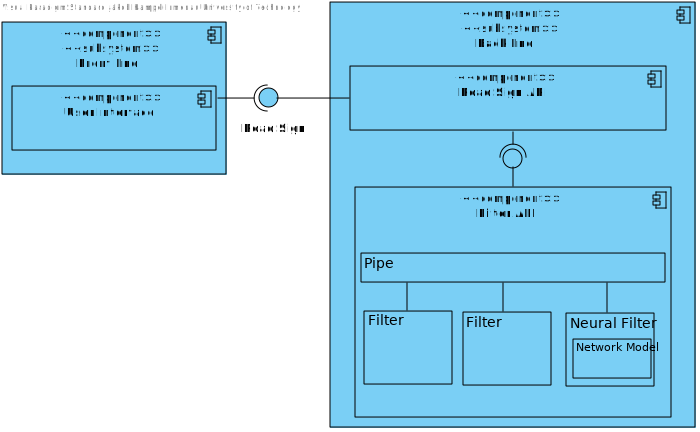
\includegraphics[width=0.6\linewidth]{Reviewdokument/Grafiken/Component_Diagram.png}
    \caption{UML-Diagramm der Subsystemstruktur}
	\label{fig:subsys}
\end{figure}

Die einzelnen Subsysteme bzw. Komponenten seien im Folgenden näher erläutert.

\section{Back-End}

Das Back-End der Anwendung besteht aus der \gls{Filter-API}, welche nach dem \glslink{Pipes and Filters}{Pipes-and-Filters-Prinzip} klassische Algorithmen oder \glslink{Neuronales Netzwerk}{Neuronale Netzwerke} auf einer \gls{Pipe} registriert. Im Folgenden werden diese \gls{Filter} bzw. \glslink{Neuronaler Filter}{Neuronale Filter} genannt.

\subsection{Filter-API}
\label{subsec:detec-api}

\begin{longtabu}{l X[j]}
{[S211]} & Die \gls{Filter-API} wird den Kern des Back-Ends des \gls{System}s darstellen.\\
&\\
{[S212]} & Basierend auf \glqq \gls{Pipes and Filters}\grqq{}-Architektur soll die \gls{Filter-API} alle \gls{Filter} und Neuronalen Filter verwalten. Näheres dazu unter [S215], [S216] und [S217].\\
&\\
{[S213]} & Die \gls{Filter-API} kann einstellbar viele \gls{Pipe} besitzen, auf der \gls{Filter} registriert werden können.\\
&\\
{[S214]} & Die \gls{Filter-API} soll Bilder entgegennehmen und darauf die entsprechenden \gls{Filter} anwenden, wobei Metainformationen wie z.B. die Position eines erkannten Objektes im Bild, erzeugt werden. Diese Metainformationen können ggf. in der weiteren Verarbeitung verwendet werden.\\
&\\
{[S215]} & Ein \gls{Filter} im Sinne der \gls{Filter-API} ist eine Klasse, die eine Methode implementiert, welche ein Bild (ggf. mit Metainformationen) entgegennimmt, diese jeweils bearbeitet und wieder an die \gls{Pipe} übergibt.\\
&\\
{[S216]} & Von der Basisklasse \gls{Filter} sollen Unterklassen abgeleitet werden können, sodass sich beliebige \gls{Filter} implementieren lassen werden.\\
&\\
{[S217]} & Ein standardmäßig implementierter \gls{Filter} ist der \glslink{Neuronaler Filter}{Neuronale Filter}, welcher Filterfunktionen auf Basis \glslink{Neuronales Netzwerk}{Neuronaler Netzwerke} anwendet. Näheres dazu im Entwurfsdokument.\\
\end{longtabu}

\subsection{Verkehrszeichen-API}

\begin{longtabu}{l X[j]}
{[S221]} & Die \gls{Verkehrszeichen-API} soll die \gls{Filter-API} benutzen, um die entsprechend benötigten \gls{Filter} zur Verkehrszeichenerkennung zu definieren und zu verwalten.\\
&\\
{[S222]} & Sie kann dabei ein Einzelbild oder eine Serie aus Bildern entgegennehmen und an die \gls{Filter-API} übergeben. Entsprechend der Bewertung durch diese werden die erkannten Schilder zurückgegeben.
\end{longtabu}
\end{comment}

\begin{appendix}

\chapter{Sonstiges}
\section{Zu erkennenden Verkehrzeichen-Klassen}
\label{sec:list_classes}
\begin{longtabu}{X[l] X[l]}
\hline
\bf Klasse & \bf Entsprechende Verkehrszeichen und -gruppen \\ \hline
Geschwindigkeitsbegrenzungen & \gls{VZ} 274 \\ \hline
Ende der Geschwindigkeitsbegrenzungen & \gls{VZ} 278, \gls{VZ} 282 \\ \hline
Vorgeschriebene Mindestgeschwindigkeit & \gls{VZ} 275 \\ \hline
Ende der vorgeschriebenen Mindestgeschwindigkeit & \gls{VZ} 279, \gls{VZ} 282 \\ \hline
Anlagenzeichen & \gls{VZ} 310, \gls{VZ} 311, \gls{VZ} 325, \gls{VZ} 330, \gls{VZ} 331 \\ \hline
Fahrschstreifentafeln & \gls{VZ} 523, \gls{VZ} 525, \gls{VZ} 526 \\ \hline
Zusatzzeichen & \gls{VZ} 1001, \gls{VZ} 1004, \gls{VZ} 1040, \gls{VZ} 1042, \gls{VZ} 1053	\\ \hline
\hline
\end{longtabu}

\section{Zu erkennenden Verkehrzeichen}
\label{sec:liste_zu_erkennende_verkehrszeichen}
Hier werden alle Verkehrszeichen gelistet, welche erkannt werden müssen, um den \gls{Nutzer} fehlerfrei auf eventuelle Geschwindigkeitsüber- oder unterschreitungen aufmerksam zu machen.

\begin{longtabu}{l X[j]}
\hline
\bf Nummerierung & \bf Bezeichnung\\
\hline
\gls{VZ}	274-5	&  	zulässige Höchstgeschwindigkeit 5 km/h\\ 
\hline
\gls{VZ}	274-10	& zulässige Höchstgeschwindigkeit 10 km/h\\ \hline
\gls{VZ}	274-20	& zulässige Höchstgeschwindigkeit 20 km/h\\ \hline
\gls{VZ}	274-30	& zulässige Höchstgeschwindigkeit 30 km/h\\ \hline
\gls{VZ}	274-40	& zulässige Höchstgeschwindigkeit 40 km/h\\ \hline
\gls{VZ}	274-50	& zulässige Höchstgeschwindigkeit 50 km/h\\ \hline
\gls{VZ}	274-60	& zulässige Höchstgeschwindigkeit 60 km/h\\ \hline
\gls{VZ}	274-70	& zulässige Höchstgeschwindigkeit 70 km/h\\ \hline
\gls{VZ}	274-80	& zulässige Höchstgeschwindigkeit 80 km/h\\ \hline
\gls{VZ}	274-90	& zulässige Höchstgeschwindigkeit 90 km/h\\ \hline
\gls{VZ}	274-100	& zulässige Höchstgeschwindigkeit 100 km/h\\ \hline
\gls{VZ}	274-110	& zulässige Höchstgeschwindigkeit 110 km/h\\ \hline
\gls{VZ}	274-120	& zulässige Höchstgeschwindigkeit 120 km/h\\ \hline
\gls{VZ}	274-130	& zulässige Höchstgeschwindigkeit 130 km/h\\ \hline
\gls{VZ}	274.1	& Beginn einer Tempo 30-Zone\\ \hline
\gls{VZ}	274.1-20& Beginn einer Tempo 20-Zone\\ \hline
\gls{VZ}	274.2	& Ende einer Tempo 30-Zone\\ \hline
\gls{VZ}	274.2-20& Ende einer Tempo 20-Zone\\ \hline
\gls{VZ}	275-5	& Vorgeschriebene Mindestgeschwindigkeit 5 km/h\\ \hline
\gls{VZ}	275-10	& Vorgeschriebene Mindestgeschwindigkeit 10 km/h\\ \hline
\gls{VZ}	275-20	& Vorgeschriebene Mindestgeschwindigkeit 20 km/h\\ \hline
\gls{VZ}	275-30	& Vorgeschriebene Mindestgeschwindigkeit 30 km/h\\ \hline
\gls{VZ}	275-40	& Vorgeschriebene Mindestgeschwindigkeit 40 km/h\\ \hline
\gls{VZ}	275-50	& Vorgeschriebene Mindestgeschwindigkeit 50 km/h\\ \hline
\gls{VZ}	275-60	& Vorgeschriebene Mindestgeschwindigkeit 60 km/h\\ \hline
\gls{VZ}	275-70	& Vorgeschriebene Mindestgeschwindigkeit 70 km/h\\ \hline
\gls{VZ}	275-80	& Vorgeschriebene Mindestgeschwindigkeit 80 km/h\\ \hline
\gls{VZ}	278-5	& Ende der zulässigen Höchstgeschwindigkeit 5 km/h\\ \hline
\gls{VZ}	278-10	& Ende der zulässigen Höchstgeschwindigkeit 10 km/h\\ \hline
\gls{VZ}	278-20	& Ende der zulässigen Höchstgeschwindigkeit 20 km/h\\ \hline
\gls{VZ}	278-30	& Ende der zulässigen Höchstgeschwindigkeit 30 km/h\\ \hline
\gls{VZ}	278-40	& Ende der zulässigen Höchstgeschwindigkeit 40 km/h\\ \hline
\gls{VZ}	278-50	& Ende der zulässigen Höchstgeschwindigkeit 50 km/h\\ \hline
\gls{VZ}	278-60	& Ende der zulässigen Höchstgeschwindigkeit 60 km/h\\ \hline
\gls{VZ}	278-70	& Ende der zulässigen Höchstgeschwindigkeit 70 km/h\\ \hline
\gls{VZ}	278-80	& Ende der zulässigen Höchstgeschwindigkeit 80 km/h\\ \hline
\gls{VZ}	278-90	& Ende der zulässigen Höchstgeschwindigkeit 90 km/h\\ \hline
\gls{VZ}	278-100	& Ende der zulässigen Höchstgeschwindigkeit 100 km/h\\ \hline
\gls{VZ}	278-110	& Ende der zulässigen Höchstgeschwindigkeit 110 km/h\\ \hline
\gls{VZ}	278-120	& Ende der zulässigen Höchstgeschwindigkeit 120 km/h\\ \hline
\gls{VZ}	278-130	& Ende der zulässigen Höchstgeschwindigkeit 130 km/h\\ \hline
\gls{VZ}	279-5   & Ende der vorgeschriebenen Mindestgeschwindigkeit 5 km/h\\ \hline
\gls{VZ}	279-10  & Ende der vorgeschriebenen Mindestgeschwindigkeit 10 km/h\\ \hline
\gls{VZ}	279-20	& Ende der vorgeschriebenen Mindestgeschwindigkeit 20 km/h\\ \hline
\gls{VZ}	279-30	& Ende der vorgeschriebenen Mindestgeschwindigkeit 30 km/h\\ \hline
\gls{VZ}	279-40	& Ende der vorgeschriebenen Mindestgeschwindigkeit 40 km/h\\ \hline
\gls{VZ}	279-50	& Ende der vorgeschriebenen Mindestgeschwindigkeit 50 km/h\\ \hline
\gls{VZ}	279-60	& Ende der vorgeschriebenen Mindestgeschwindigkeit 60 km/h\\ \hline
\gls{VZ}	279-70	& Ende der vorgeschriebenen Mindestgeschwindigkeit 70 km/h\\ \hline
\gls{VZ}	279-80	& Ende der vorgeschriebenen Mindestgeschwindigkeit 80 km/h\\ \hline
\gls{VZ}	282	    & Ende sämtlicher Streckenverbote\\ \hline
\gls{VZ}	310	    & Ortstafel Vorderseite (\glqq{}Ortseingangsschild\grqq)\\ \hline
\gls{VZ}	311	    & Ortstafel Rückseite (\glqq{}Ortsausgangsschild\grqq)\\ \hline
\gls{VZ}	325.1	& Beginn eines verkehrsberuhigten Bereichs\\ \hline
\gls{VZ}	325.2	& Ende eines verkehrsberuhigten Bereichs\\ \hline
\gls{VZ}	330.1	& Autobahn\\ \hline
\gls{VZ}	330.2	& Ende der Autobahn\\ \hline
\gls{VZ}	331.1	& Kraftfahrstraße\\ \hline
\gls{VZ}	331.2	& Ende der Kraftfahrstraß\\ \hline
\gls{VZ}	523-30	& Fahrstreifentafel ohne Gegenverkehr - zweistufig (Höchstgeschwindigkeit)\\ \hline
\gls{VZ}	523-31	& Fahrstreifentafel ohne Gegenverkehr - dreistreifig (Höchstgeschwindigkeit)\\ \hline
\gls{VZ}	525-31	& Fahrstreifentafel ohne Gegenverkehr (Mindestgeschwindigkeit) - zweistreifig\\ \hline
\gls{VZ}	 526-31	& Fahrstreifentafel mit Gegenverkehr - zweistreifig in Fahrtrichtung und einstreifig in Gegenrichtung (Mindestgeschwindigkeit)\\ \hline
\gls{VZ}	 526-33	& Fahrstreifentafel mit Gegenverkehr - zweistreifig in Fahrtrichtung und zweistreifig in Gegenrichtung (Mindestgeschwindigkeit)\\ \hline
\gls{VZ}	1001-30	& auf ... m \\ \hline
\gls{VZ}	1001-31	& auf ... km \\ \hline
\gls{VZ}	1001-33	& noch ... km \\ \hline
\gls{VZ}	1001-34	& auf ... m \\ \hline
\gls{VZ}	1001-35	& auf ... km \\ \hline
\gls{VZ}	1004-30	& nach ... m \\ \hline
\gls{VZ}	1004-31	& in ... km \\ \hline
\gls{VZ}	1040-30	& zeitliche Beschränkung (16-18 h) \\ \hline
\gls{VZ}	1040-31	& zeitliche Beschränkung (8-11 h, 16-18 h) \\ \hline
\gls{VZ}	1040-34	& ab Zeitpunkt \\ \hline
\gls{VZ}	1040-35	& Lärmschutz mit Zeitangabe \\ \hline
\gls{VZ}	1040-36	& Schulweg in Verbindung mit zeitlicher Begrenzung \\ \hline
\gls{VZ}	1042-30	& werktags \\ \hline
\gls{VZ}	1042-31	& werktags 18-19 h \\ \hline
\gls{VZ}	1042-32	& werktags 8.30-11.30 h, 16-18 h \\ \hline
\gls{VZ}	1042-33	& Mo-Fr, 16-18 h \\ \hline
\gls{VZ}	1042-34	& Di, Do, Fr, 16-18 h \\ \hline
\gls{VZ}	1042-35	& 6-22 h an Sonn- und Feiertagen \\ \hline
\gls{VZ}	1042-38	& werktags außer samstags \\ \hline
\gls{VZ}	1042-51	& Sa und So	\\ \hline
\gls{VZ}	1042-53	& Schulweg in Verbindung mit zeitlicher Begrenzung an Werktagen	\\ \hline
\gls{VZ}	1053-35	& bei Nässe	\\ \hline

\end{longtabu}

\printnoidxglossary[type=\acronymtype,numberedsection=autolabel] 

\end{appendix}
\end{document}
